%    Figure insertion; default placement is top; if the figure occupies
%    more than 75% of a page, the [p] option should be specified.
\begin{table}[t]
	\begin{center}
		\begin{tabular}{ccc}
		  %
		  $\U{}$ & $\sig{}$ & $\V{*}$ \\[5pt]
		  %
	 	  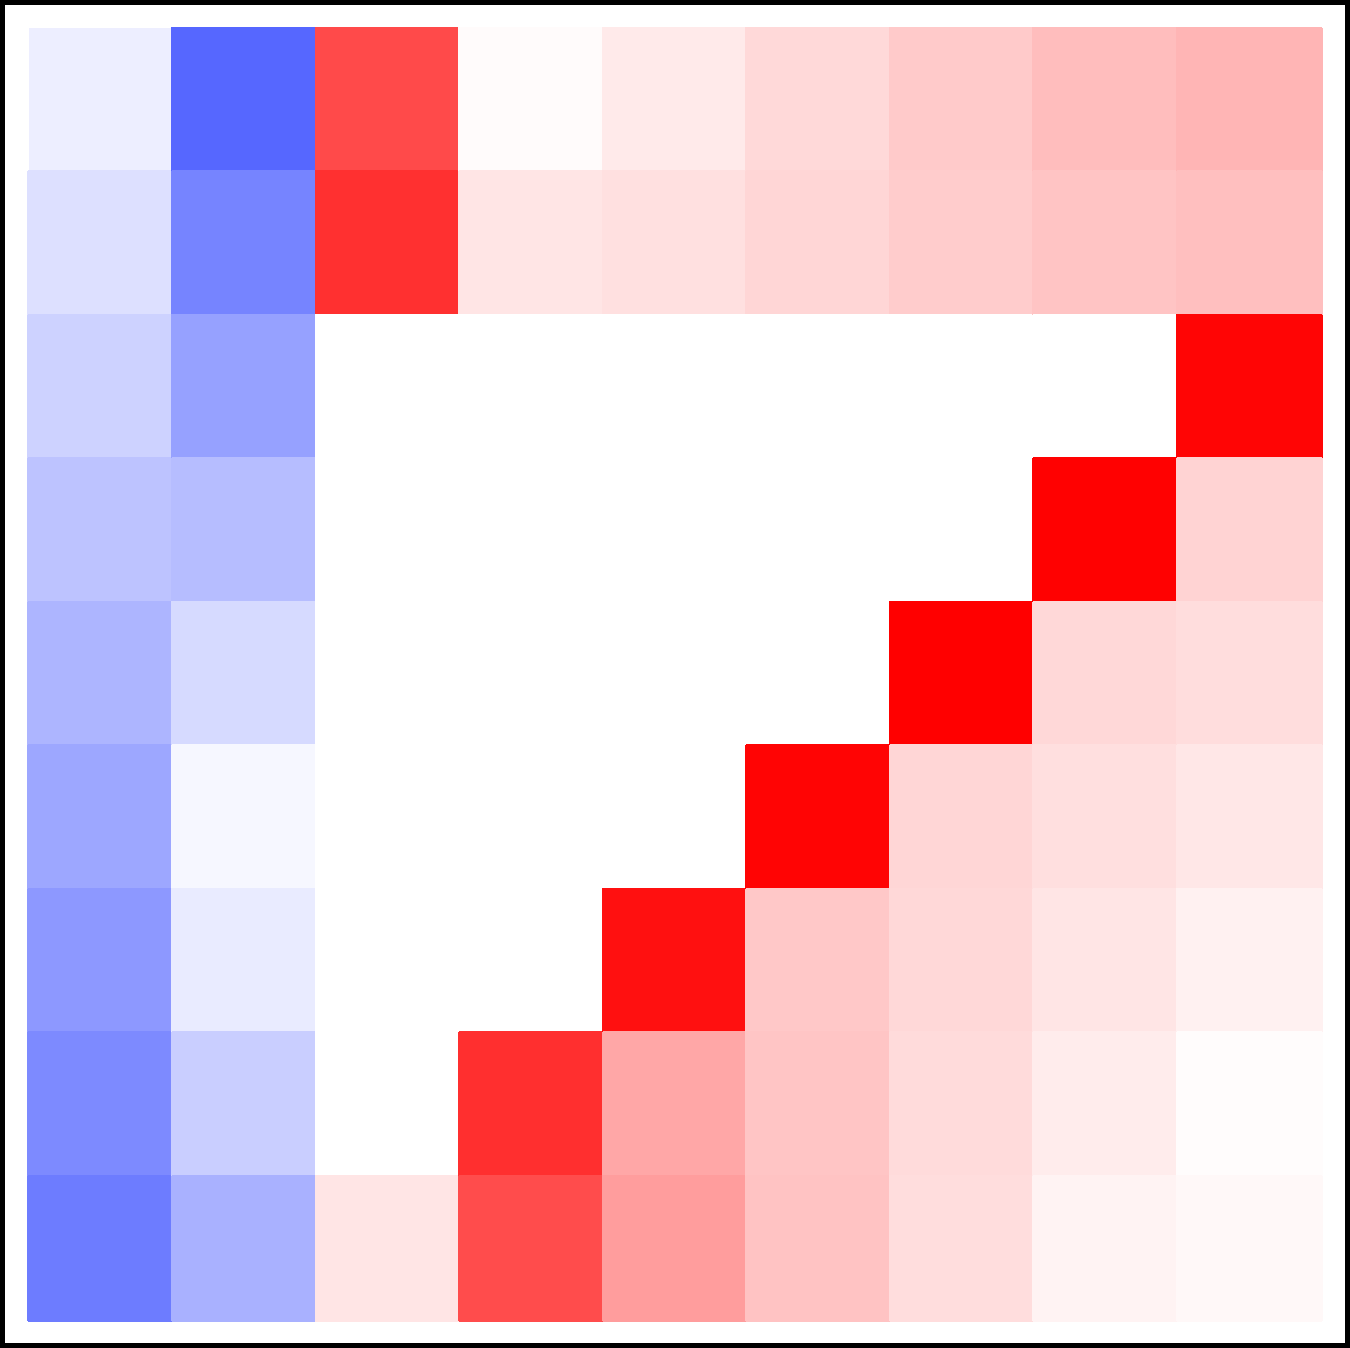
\includegraphics[ width = 9cm ]{\pathgraphics "bevington poles"/U}  &
		  
\includegraphics[ width = 2.075cm ]{\pathgraphics "bevington poles"/S}  &
		  \raisebox{3.5\height}{\includegraphics[ width = 2cm ]{\pathgraphics "bevington poles"/Vt} }\\
		  %
		\end{tabular}
	\end{center}
	\label{tab:bevington usv block}
	\caption[Decomposition for the system matrix $\A{}$]{Decomposition for the system matrix $\A{}$. Column vectors of codomain matrix $\U{}=\cublockf$ span the space $\cmplx{9}$; the blue vectors are a span for $\brnga{}$, red for $\rnlla{*}$. The brightest colors represent an entry of unit magnitude; white signifies a 0 entry. The $\sig{}$ matrix is shown in gray scale because neither column nor row vector lie in a range or null space. This matrix contains the matrix of singular values $\ess{}$ in a sabot matrix of zeros for shape arbitration. The final matrix $\U{*}$ represents the domain. As the problem is full rank there is no null space $\rnlla{*}$ and the column vectors represent a complete space of $\brnga{*}$.}
\end{table}%

\endinput  %  -  -  -  -  -  -  -  -  -  -  -  -  -  -  -  -  -  -  -  -

%\input{\pathtables "tab XXX"}  %  <  <  <  <  <  <  <  <  <  <  <  <